\documentclass{article}
\usepackage{amsmath}
\usepackage{tikz}
\usepackage{tkz-euclide}
\usepackage{amsfonts}
\usepackage{graphicx}
\graphicspath{{./assets/}}

\numberwithin{equation}{section}
\title{Gravity Demo}
\author{Martin N. Håvardsen}
\date{\today}

\begin{document}
\maketitle
\begin{center}
\includegraphics[width=0.8\textwidth]{ARTSTYLE.png}\\
\end{center}
\section{Generell protokoll}
Prosesson for simuleringen per objekt skal gå som følger:
\begin{itemize}
  \item tegn
  \item kalkuler akselerasjon
  \item kalkuler fart
  \item kalkuler posisjon
  \item oppdater alle egenskaper --- poisjon, fart og akselerasjon
\end{itemize}
\section{Objekt}
\subsection{Egenskaper}
alle objekt skal ha følgende egenskaper:
\begin{itemize}
  \item posisjon
  \item fart
  \item akselerasjon
  \item masse
\end{itemize}
\subsection{Teori for å kalkulere akselerasjon}
For et objekt~$A$ med masse $m_A$ og distansen r til et objekt~$B$, så vil kraften $G_B$ som $B$ påfører $A$ vil være gitt ved følgende:
\begin{equation}
  G_B=\gamma\frac{m_Am_B}{r_B^2}
  \label{eq:gravitasjonskraft}
\end{equation}
Gravitasjonskonstanten, $\gamma$, vil være en svært liten konstant. \\ 
Fra Newtons andre lov får vi at akselerasjonen til objekt $A$, $\vec a=\displaystyle\frac {\overrightarrow{\Sigma F}} {m_A}$. Siden $\overrightarrow{\Sigma F}=\vec G_B+\vec G_C+\dots$, for gravitasjonskrefter fra andre objekt $B$, $C$ osv. $\overrightarrow{\Sigma F}$ kommer bare til å bestå av gravitasjonskrefter i denne simuleringen.
\begin{align}
  \vec a &= \frac{\hat {G}_B\cdot\gamma\frac{m_Am_B}{r_B^2}+\hat {G}_C\cdot\gamma\frac{m_Am_C}{r_C^2}+\dots }{m_A}\\
  \vec a &=\gamma\left(\frac {\hat{G}_B \cdot m_B} {r_B^2}+\frac {\hat{G}_C\cdot m_C} {r_C^2}\right)
\end{align}
$\hat G_B$ vil alltid være rettet mot $B$, fra $A$. 
\begin{equation}
  \hat G_B=\frac{\vec s_B-\vec s_A}{r}
  \label{eq:G_enhet}
\end{equation}
\subsection{Metode for å kalkulere akselerasjon}
\begin{enumerate}
  \item Finn alle retningsvektorer for gravitasjonskreftene.
  \item Regn ut $\vec a$ 
\end{enumerate}
Her er hvordan dette ble implementert:\\
\includegraphics[width=1\textwidth]{update_acceleration_CODE.png}
\texttt{obj} her er et \texttt{PhysObj} objekt som inneholder sin masse, posisjon, fart og akselerasjon. Denne funksjonen utføres en gang per \textit{frame} for hvert objekt.
%\eqref{eq:gravitasjonskraft}
\section{Perspektiv og koordinatsystem}
\subsection{Mål}
Simuleringen skal ha kamerafunksjonalitet. Man skal kunne bevege koordinatsystemet/rutenettet med musen --- bevege \textit{kameraet}. I tillegg skal det være mulig å forstørre rutenettet --- \textit{zoome}.
\subsection{Teori}
Planet som objektene tilhører, er kartesisk og har to dimensjonene. Disse dimensjonene kan fremstilles med to retningsvektorer, $\hat i, \hat j$, som --- skalert, kan kombineres til å få hva som helst punkt på planet.\\ 
Koordinaten i vinduet som objektet blir tegnet i er ikke nødvendigvis lik koordinaten på planet. Hvordan transformeringen av romkoordinaten til vinduskoordinat skjer kan variere. Relevante faktorer her er \textit{kameraet} sin posisjon, eventuell \textit{zoom}, og \textit{rotasjon}. Her ignorerer vi rotasjon. \\ 
Vi har da at transformeringen $T:\mathbb{R}^2 \to \mathbb{R}^2$, \\
%\begin{tikzpicture}
%  \draw[->] (0,0) -- (3,0) node[right] {$x$};
%  \draw[->] (0,0) -- (0,2) node[above] {$y$};
%  \draw[step=0.5cm,gray,very thin] (-1,-1) grid (4,3);
%  \draw[thick, blue] (0,0) -- (2,1) node[midway, above] {$\vec{v}$};
%  % Points and vectors 
%  \filldraw[blue] (0,0) circle (1pt) node[below left] {$O$};
%  \filldraw[red] (2,1) circle (1pt) node[above right] {$A(2,1)$};
%\end{tikzpicture}
\begin{figure}[h]
\centering
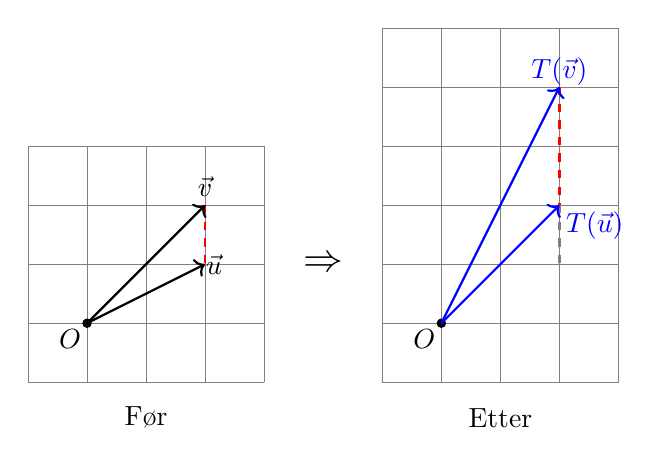
\begin{tikzpicture}[scale=1.5, every node/.style={inner sep=0pt}]
  % Left picture
  \begin{scope}[shift={(0,0)}]
    \draw[step=0.5cm,gray,very thin] (-0.5,-0.5) grid (1.5,1.5);
    \draw[dashed, thick, red] (1,1) -- (1,0.5);
    \filldraw[black] (0,0) circle (1pt) node [below left=0.1] {$O$};
    \draw[thick,->] (0,0) -- (1,1) node[above=0.1cm] {$\vec{v}$};
    \draw[thick,->] (0,0) -- (1,0.5) node[right] {$\vec{u}$};
    \node at (0.5,-0.8) {Før};
  \end{scope}

  % Arrow in the middle
  \node at (2,0.5) {\Large $\Rightarrow$};

  % Right picture
  \begin{scope}[shift={(3,0)}]
    \draw[step=0.5cm,gray,very thin] (-0.5,-0.5) grid (1.5,2.5);
    \draw[dashed, thick, red] (1,2) -- (1,1);
    \draw[dashed, thick, gray] (1,1) -- (1,0.5);
    \filldraw[black] (0,0) circle (1pt) node [below left=0.1cm] {$O$};
    \draw[thick,->,blue] (0,0) -- (1,2) node[above] {$T(\vec{v})$};
    \draw[thick,->,blue] (0,0) -- (1,1) node[below right=0.1cm] {$T(\vec{u})$};
    \node at (0.5,-0.8) {Etter};
  \end{scope}
\end{tikzpicture}
  \caption{Transformeringen av $\vec v$ og $\vec u$ under $T$}
\end{figure}
\begin{equation}
%\begin{bmatrix}v_x \\ v_y\end{bmatrix}
  T(\vec v)=k\vec v+ \vec c
  \label{eq:transformeringen}
\end{equation}
Musehjulet skal da forandre $k$ fra \eqref{eq:transformeringen}, dette vil forstørre/forminske rutenettet. Merk at $k\in \langle 0, \infty\rangle$ \\
$\vec c$ fra \eqref{eq:transformeringen} er koordinaten på planet som tilsvarer \texttt{(0,0)} i vinduet.
Vi finner også den inverse transformeringen ved:
\begin{equation}
  T^{-1}(\vec v)=\frac{\vec v-\vec c}{k}=\frac 1 k \vec v-\frac 1 k\vec c
  \label{eq:invers transformeringen}
\end{equation}
$T^{-1}(\vec v)$ vil da være koordinaten i vinduet som tilsvarer koordinaten på planet.
\section{Kollisjon}
\subsection{Objekt vs barriere}
% collision drawing
\begin{figure}[h]
  \centering
  \begin{tikzpicture}[scale=1]
    \begin{scope}[shift={(0,0)}]
      \begin{scope}[shift={(0,-0.4)}, rotate=30]
        \draw (0,0) circle (1) node[left]{$A$};
        \draw [thin, ->, blue] (-0.8,1.2) -- (0.8,1.2) node[midway, above=0.1]{$\vec v_{A0}$};
      \end{scope}[rotate=30]
      \draw [thick, red] (2,2) -- (2,-1) node[above right=0.1]{$B$};
      \node[scale=1, circle] (B) at (0,-2){Før};
    \end{scope}
    %\node[scale=2, circle] (A) at (4,0){$\implies$};
    \begin{scope}[shift={(4.5,0)}]
      \begin{scope}[shift={(1,0.4)},rotate=30]
        \draw (0,0) circle (1) node[left]{$A$};
        %\draw [thin, ->, blue] (-1.2,-1.2) -- (0.4,-1.2) node[midway, below]{$\vec v_{A0}$};
      \end{scope}[rotate=30]
      % Triangle points
      \coordinate (A1) at (0,0);
      \coordinate (B1) at (4,0);
      \coordinate (C1) at (2,3);
      \draw [thick, red] (2,2) -- (2,-1) node[above right=0.1]{$B$};
      \node[scale=1, circle] (B) at (0.8,-2){Under kontakt};
    \end{scope}
    \begin{scope}[shift={(9.5,0)}]
      \begin{scope}[shift={(0,1.2)}, rotate=-30, xscale=-1]
        \draw (0,0) circle (1) node[left]{$A$};
        \draw [thin, ->, blue] (-0.8,1.2) -- (0.8,1.2) node[midway, above]{$\vec v_A$};
      \end{scope}
      \draw [thick, red] (2,2) -- (2,-1) node[above right=0.1]{$B$};
      \node[scale=1, circle] (B) at (0.4,-2){Etter};
    \end{scope}
  \end{tikzpicture}
  \caption{Kollisjon mellom objekt $A$ og barriere $B$}
\end{figure}
\begin{align}
  \vec\rho_{A0}+\vec\rho_{B0}&=\vec\rho_{A}+\vec\rho_{B}
  \label{eq:bevaring av bevegelsesmengde} \\
  \|\vec\rho_{B0}\| = \rho_{B0} = 0 \implies\vec\rho_{A0}&=\vec\rho_{A}+\vec\rho_{B}
  \label{eq:impl bvgmngd}
\end{align}
La kinetisk energi, $E_k$, bevares, $E_{k0}=E_k$
\begin{align}
  E_{kA0}+E_{kB0}&=E_{kA}+E_{kB} \\
  \frac 1 2 m_A v_{A0}+\frac 1 2 m_B v_{B0}&=\frac 1 2 m_A v_{A}+\frac 1 2 m_B v_{B}\\
  m_A v_{A0}-m_A v_{A} &= m_B v_{B}-m_B v_{B0}\\
  m_A(v_{A0}-v_{A}) &= m_B(v_{B}-v_{B0}) \\
  -\Delta\rho_A &= \Delta\rho_B
\end{align}
Vi vet at $v_B=0$. Derfor må $\Delta\rho_A=0$. Siden barrieren kun kan utøve en kraft som ligger normalt til barriereplanet, så vil $\vec v_A=\vec v_{A0}+\vec N_{normal}$. Dette vil si at siden bevegelsesmengden er bevart for $A$, så vil innfalsvinkelen og utfallsvinkelen være like.
\begin{figure}[h]
  \centering
  \begin{tikzpicture}[scale=1]
    \coordinate (A1) at (-5,2);
    \coordinate (A2) at (-5,-2);
    \coordinate (O) at (0,0);
    \coordinate (B1) at (5,2);
    \coordinate (B2) at (5,-2);
    \coordinate (E1) at (-5,0);
    \coordinate (E2) at (5,0);
    \draw[red, thick, ->] (O) -- (0,1) node[above, right]{$\vec n$};
    \draw[blue] (A1) -- (O);
    \draw[blue, thick, ->] (A1) -- ($(A1)!0.4!(O)$) node[above, right]{$\vec v_{A0}$};
    \draw[blue, dashed] (O) -- (B1);
    \draw[blue, dashed] (O) -- (B2);
    \draw (E1) -- (E2);
    \pic["$\alpha$", draw, angle radius=1.6cm] {angle = A1--O--E1};
    \pic["$\beta$", draw, angle radius=1.6cm, dashed] {angle = E2--O--B1};
  \end{tikzpicture}
  \caption{Speiling}
\end{figure}
\subsection{Objekt vs Objekt}
\section{Program struktur}
\subsection{Globale variabler}
\begin{itemize}
  \item \texttt{SCREEN\_WIDTH = 1280}
  \item \texttt{SCREEN\_HEIGHT = 720}
  \item \texttt{FPS\_TARGET = 180}
  \item \texttt{screen = pygame.display.set\_mode((SCREEN\_WIDTH, SCREEN\_HEIGHT))}
  \item \texttt{pygame.display.set\_caption("Gravity Demo")}
  \item \texttt{font = pygame.font.Font(None, 36)}
  \item \texttt{clock = pygame.time.Clock()}
  \item \texttt{meters\_per\_screenwidth = 150E9*2}
  \item \texttt{k\_meters\_per\_pixel = meters\_per\_screenwidth/SCREEN\_WIDTH }
  \item \texttt{k\_increment = k\_meters\_per\_pixel*0.05}
  \item \texttt{c\_coordinate\_at\_origin = pygame.Vector2(0,0)}
  \item \texttt{mouse\_drag\_start = pygame.Vector2(-1,-1)}
  \item \texttt{global\_mb2\_down = False}
  \item \texttt{object\_size\_pixels = 100}
  \item \texttt{RUNNING = True}
  \item \texttt{GAMMA = 7E-11}
  \item \texttt{R\_RELATIVE\_TO\_M=False}
  \item \texttt{objA = PhysObj(...)}
  \item \texttt{objB = PhysObj(...)}
  \item \texttt{objC = PhysObj(...)}
  \item \texttt{objD = PhysObj(...)}
  \item \texttt{ALL\_OBJECTS = [objA, objB, objC, objD]}
\end{itemize}
\subsection{Funksjoner}
\begin{table}[h]
  \centering
  \begin{tabular}{|l|l|l|}
  \hline
  \textbf{Funksjon} & \textbf{input} &\textbf{output} \\
  \hline
  \texttt{update\_objects} &  & \\
  \hline
    \texttt{add\_object\_with\_vel} &\texttt{pos} : \textit{vec2}&\\& \texttt{color} : \textit{vec3}&\\& \texttt{mass} : \textit{float}&\\& \texttt{vel} : \textit{vec2} & \\
  \hline
    \texttt{add\_object} &\texttt{pos} : \textit{vec2}&\\& \texttt{color} : \textit{vec3}&\\& \texttt{mass} : \textit{float}& \\
  \hline
  \texttt{transform\_window\_to\_plane} &\texttt{v} : \textit{vec2} & transformed v \\
  \hline
  \texttt{transform\_plane\_to\_window} &\texttt{v} : \textit{vec2} &transformed v \\
  \hline
    \texttt{transform\_plane\_to\_window\_tuplet} &\texttt{v} : \textit{vec2}  & transformed v\\
  \hline
    \texttt{draw\_circle\_in\_plane} &\texttt{window} : \textit{pygame.surface}&\\& \texttt{color} : \textit{vec3}&\\& \texttt{pos} : \textit{vec2}&\\& \texttt{rad} : \textit{uint}&\\& \texttt{outline\_thickness} : \textit{uint} & \\
  \hline
  \texttt{handle\_mb2} & & \\
  \hline
\end{tabular}
  \caption{Matrise med funksjoner}
\end{table}

\begin{itemize}
    \item \textbf{Global Scope}
    \begin{itemize}
        \item Variables: \texttt{RUNNING, MB1, MB2, MB3, MX, MY, global\_mb2\_down, object\_size\_pixels, k\_meters\_per\_pixel, k\_increment, clock, FPS\_TARGET, font, screen}
        \item Functions: \texttt{add\_object, add\_object\_with\_vel, transform\_window\_to\_plane, transform\_plane\_to\_window, handle\_mb2, update\_objects}
    \end{itemize}

    \item \textbf{Main While Loop: \texttt{while RUNNING:}}
    \begin{itemize}
        \item \textbf{Event Loop: \texttt{for event in pygame.event.get():}}
        \begin{itemize}
            \item \texttt{if event.type == pygame.QUIT:} set \texttt{RUNNING = False}
            \item \texttt{if event.type == pygame.KEYDOWN:}
            \begin{itemize}
                \item \texttt{if key == K\_s:} update \texttt{object\_size\_pixels} from input
            \end{itemize}
            \item \texttt{if event.type == pygame.MOUSEBUTTONDOWN:}
            \begin{itemize}
                \item Read mouse buttons: \texttt{MB1, MB2, MB3} and position \texttt{MX, MY}
                \item \texttt{if MB1:} input mass, compute color, call \texttt{add\_object()}
                \item \texttt{if MB3:} input mass/velocity, compute color, call \texttt{add\_object\_with\_vel()}
                \item \texttt{if MB2:} set \texttt{global\_mb2\_down = True}
            \end{itemize}
            \item \texttt{if event.type == pygame.MOUSEWHEEL:} adjust \texttt{k\_meters\_per\_pixel} based on \texttt{event.y}
            \item \texttt{if event.type == pygame.MOUSEBUTTONUP:}
            \begin{itemize}
                \item \texttt{if MB2:} reset \texttt{global\_mb2\_down} and \texttt{mouse\_drag\_start}
            \end{itemize}
        \end{itemize}

        \item \textbf{Post-Event Loop Updates:}
        \begin{itemize}
            \item \texttt{screen.fill(pygame.Color(0,0,0))}
            \item \texttt{if global\_mb2\_down: handle\_mb2()}
            \item \texttt{update\_objects()}
            \item Render text and blit: show \texttt{k\_meters\_per\_pixel}
            \item \texttt{pygame.display.flip()}
            \item \texttt{clock.tick(FPS\_TARGET)}
        \end{itemize}
    \end{itemize}
\end{itemize}

\end{document}
\end{document}
